)\section{Überblick - Zum Beginn stand der Zufall}
\subsection{Einführung}
\subsubsection{Theorie und Reale Werte} 
Das Gebiet der \gls{g_Stochastik} beschreibt zwei Gebiete
\begin{itemize}
	\item \gls{g_Wahrscheinlichkeitstheorie}: Diese betrachtet die theoretische Modellierung von Zufallsereignissen.
	\item \gls{g_Statistik}: Dieses Gebiet versucht anhand von realen Daten Parametern und Verteilungen theoretisch modellierte Zufallsereignisse zu schätzen.
\end{itemize}


In der \gls{g_Wahrscheinlichkeitstheorie} wird angenommen, dass alle Parameter eines Zufallsexperimentes vorhanden sind. Gefragt wird, welche Ausgänge mit welcher Wahrscheinlichkeit beobachtet werden können.

\begin{center}7
	\begin{minipage}{0.75\linewidth}
		Eine Münze, die mit der Wahrscheinlichkeit $p = 0,50$ \textit{Kopf} zeigt, wird $n = 100$ geworfen. Mit welcher Wahrscheinlichkeit wird $k=60$ mal \textit{Kopf} getroffen? 
	\end{minipage}
\end{center}

\noindent In der \gls{g_Statistik} wird angenommen, dass das Zufallsexperiment schon durchgeführt wurde, jedoch dies nicht vollkommen beschrieben ist, und sein Ausgang (am Beispiel $k$) schon bekannt ist.
Gefragt wird, nach den Parametern die dieses Zufallsexperiments beschreiben, um zukünftige Ausgänge mit ihren jeweiligen Wahrscheinlichkeiten zu beschreiben.\\

\begin{center}
	\begin{minipage}{0.75\linewidth}
		Eine Münze wurde $n=100$ geworfen und hat dabei $k=60$ \textit{Kopf} angezeigt. Bestimmen (\textit{schätzen}) die Wahrscheinlichkeit $p$, mit der die Münze bei einem Wurf \textit{Kopf} zeigt.
	\end{minipage}
\end{center}

Die \gls{g_Statistik} versucht nicht Zufälligkeit aus der Welt zu eliminieren, sondern nur die Unsicherheit zu reduzieren, in welcher Welt man sich befindet.

\begin{figure}[H]
	\centering
	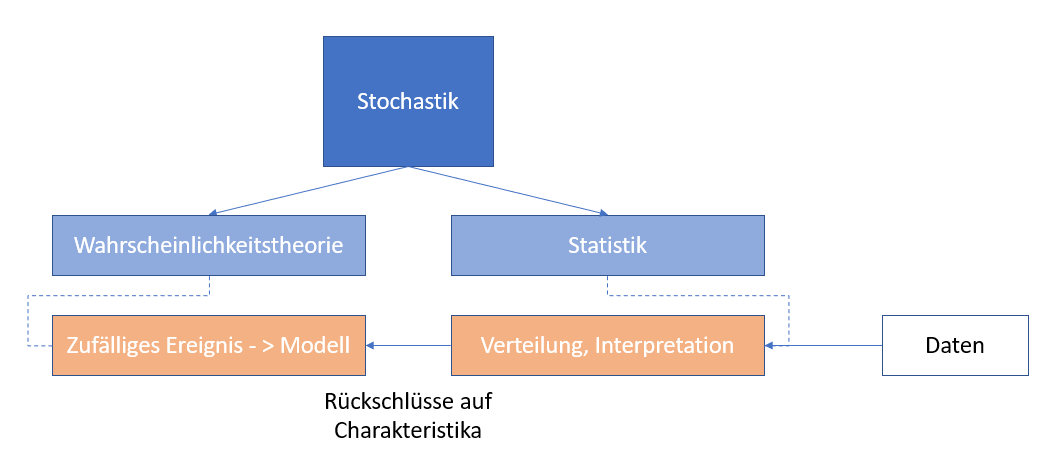
\includegraphics[scale = 0.6]{attachment/chapter_8/Scc001}
	\caption{Feld der Stochastik}
\end{figure}

Um wichtige mathematische Objekte wieder aufzufrischen, wird im Folgenden kurz das Konzept einer Abbildung erklärt.\\

\begin{itemize}
	\item In der Mathematik versteht man unter einer Abbildung oder unter gewissen Bedingungen Funktion, eine Beziehung zwischen zwei Mengen, wobei Elementen der einen Menge (Definitionsmenge, \textit{unabhängige Variablen, x-Werte, Funktionsargument}) Elementen der anderen Menge (Ergebnismenge, \textit{abhängige Variable, y-Werte, Funktionswert}) zugeordnet werden. Man spricht von einer Funktion, wenn die Abbildung in einen reelle- oder komplexwertigen Körper abbildet.\cite{Abbildung.01}
\begin{Definition}{Abbildung}
	Eine Abbildung ordnet jedem Element der Definitionsmenge $D$ genau ein Element der Zielmenge $Z$ zu: $f: D\rightarrow Z, x\mapsto y:=f(x)$
\end{Definition}
\item Die Begrifflichkeiten von Unabhängiger und Zielvarialben hat Ihren Ursprung in der Physik und Physik nahen Bereichen.
\end{itemize}

\subsubsection{Gebiete der Statistik}

Das Gebiet von Stochastik gliedert sich grob in 
\begin{description}
	\item[\gls{EDA}] Die Explorative Datenanalyse überlappt sich von der Zielsetzung mit der Deskriptiven Statistik. Es werden \textit{realen} Daten dargestellt. Ebenso werden dardurch Informationen gewonnen und Hypothesen gewonnen, welche auf das \gls{SM} schließen lassen, welche die Daten generiert. Mit dem Wachstum neuer technischer Möglichkeiten liegt der Fokus darauf, computergestützte Algorithmen zu nutzen, um Erkenntnisse über die Daten zu gewinnen. Teilaufgaben 
	\begin{itemize}
		\item wie Ausreißer finden, 
		\item Objekte mit ähnlichen Eigenschaften finden \textbf{Clusteranalyse},
		\item Kategorie schaffen \textbf{Klassifikation},
		\item stochastisch-funktionale Zusammenhängen zwischen verschiedenen Teilen der Daten zu finden \textbf{Regression},
	\end{itemize}
etc. gehen einen Schritt weiter, als die klassische \textit{Deskriptiven Statistik}.
	\item[Wahrscheinlichkeitsrechnung] Dieses Gebiet der Stochastik baut das theoretische Fundament auf, um später mit den realen Daten arbeiten zu können. Hierbei werden Werkzeug geschaffen, welche mit anderem Zweck und Bedeutung in der \textit{Deskriptiven} und \textit{Induktiven Statistik} Die \textit{Schließende Statistik} bewegt sich von den Daten und den ersten Annahmen aus, hin zu einem sicheren Verständnis, ob die getroffene Modellierung der Welt richtig ist. Dabei wird getestet, ob Hypothesen über die Annahmen der Grundgesamtheit verworfen werden müssen, oder sie den Testkriterien genügen. 
\item[Deskripten Statistik] Wie in \gls{EDA} beschrieben, ist der Zweck die Darstellung der Daten und Zusammenhänge dieser. Auch hier überlappen sich die Werkzeuge aus der \textit{Schätztheorie}, \textit{Stichprobentheorie}. Dies werden jedoch mit dem Zweck eingesetzt, erst $"$Vermutung$"$ sichtbar zu machen. 
\item[Induktiven Statistik] Die \textit{Schließende Statistik} beschäftig sich mit dem Prozess: Wenn man die Daten, Einblicke und Hypothesen über den Sachverhalt formuliert hat, wie kann man sauber eine Rückschluss auf die Grundgesamtheit (Das Theoretische Fundament) bekommen. Dabei werden unterschieden 
\begin{itemize}
	\item Stichprobentheorie, 
	\item Schätztheorie,
	\item Testtheorie
\end{itemize}
\end{description}

Die Auseinanderdividierung der Gebiet und deren Werkzeuge lässt sich somit nicht so sauber trennen, wie man es vielleicht anfänglich vermutet. Die Gebiete greifen mehr oder minder Hand in Hand, um aus 
\begin{center}
	\textit{Richtig} Daten zu erheben $\rightarrow$ Vermutungen in \textit{Statistische Modelle} umzusetzten $\rightarrow$ Erste Abschätzung über die Reale $"$modellierte$"$ Welt zu erhalten.
\end{center}


% file:///C:/Users/PaulJulitz/OneDrive%20-%20Deutsche%20Bahn/B%C3%BCcher/Mathematics/(M-AM)%20Applied/(M-AM-Sto)%20Stochastic/Mathematische%20Statistik/Skript_MaStatistik_Unbekannt.pdf
% Seite 3
%file:///C:/Users/PaulJulitz/OneDrive%20-%20Deutsche%20Bahn/B%C3%BCcher/Mathematics/(M-AM)%20Applied/(M-AM-Sto)%20Stochastic/Mathematische%20Statistik/Skript_MaStatistik_Innsbruck.pdf
%file:///C:/Users/PaulJulitz/OneDrive%20-%20Deutsche%20Bahn/B%C3%BCcher/Mathematics/(M-AM)%20Applied/(M-AM-Sto)%20Stochastic/Mathematische%20Statistik/Mathematische-Statistik_Ludenburg.pdf
% Seite 12

\begin{figure}[H]
	\centering
	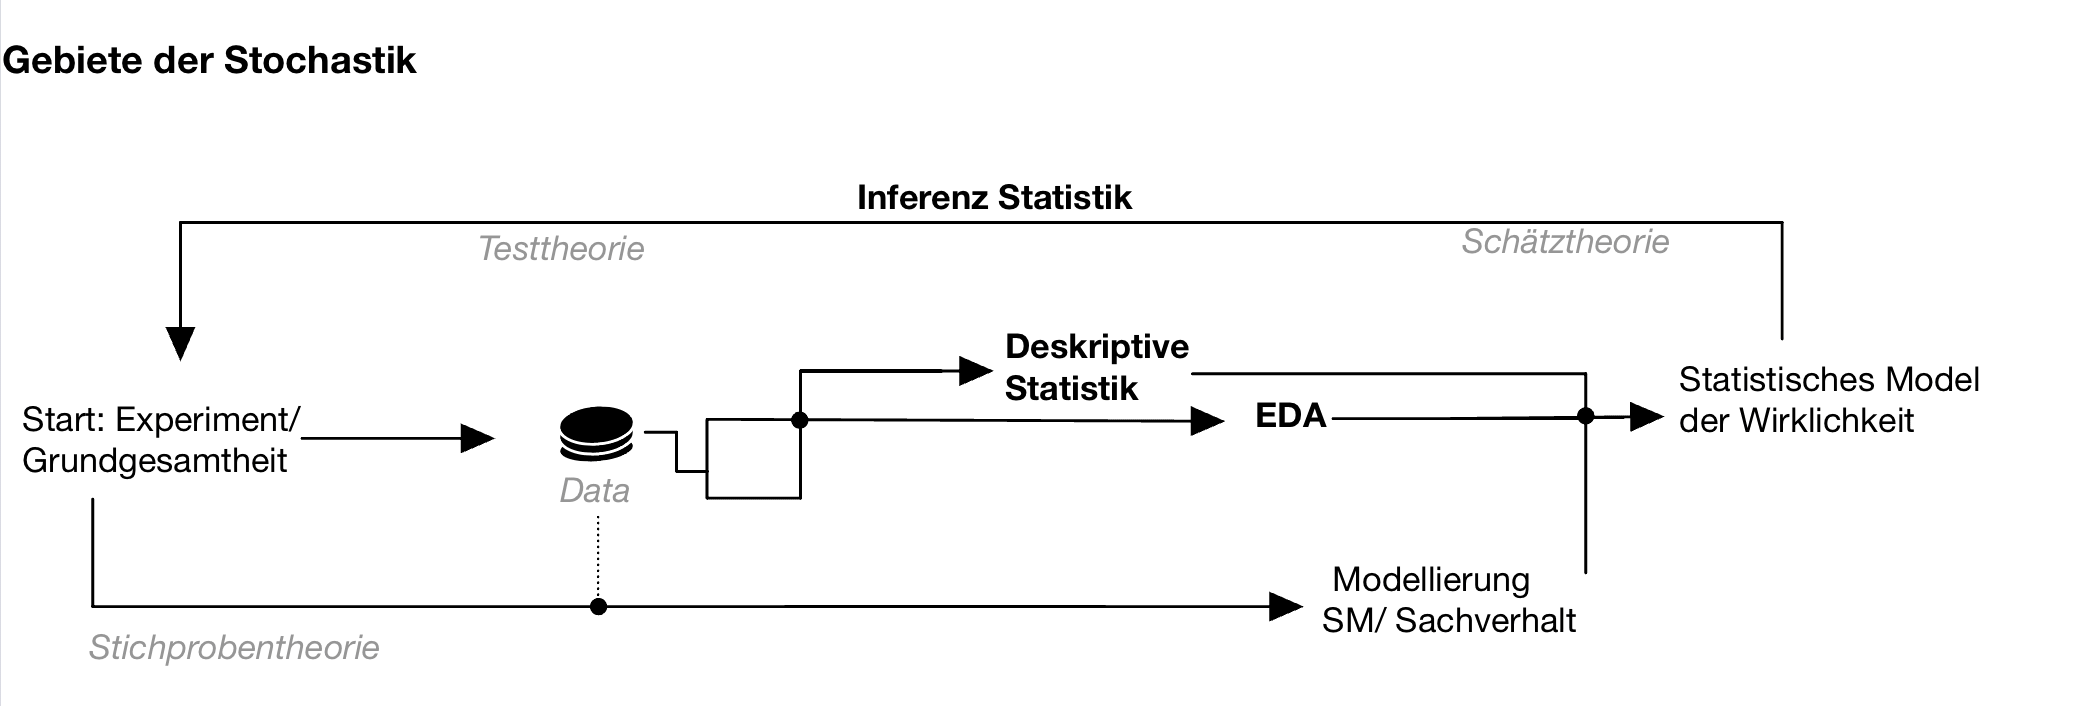
\includegraphics[width=0.7\linewidth]{attachment/chapter_13/Scc069}
	\caption{Prozess der Abbildung der Realität in eine Statisches Modell}
\end{figure}

Dabei wird mit der Stichproben aus der Grundgesamtheit der Einblick gewonnen, welcher nötig ist, um eine Rückschluss auf diese zu gewinnen.

\begin{figure}[H]
	\centering
	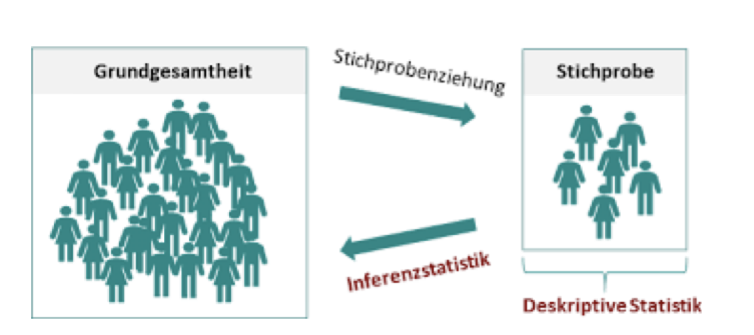
\includegraphics[width=0.5\linewidth]{attachment/chapter_13/Scc070}
	\caption{Rückschluss auf die Grundgesamtheit} 
\end{figure}

\subsubsection{Parameter der Grundgesamtheit}
Im späteren Verlauf wird sich zeigen, dass einige Werkzeuge zwischen den Teilgebieten der Deskriptiv und Induktiven Statistik in Modifikation wieder vorkommen. 

Das Gebiet von \gls{SM} beschäftigt sich ausschließlich damit, \textit{Parameter der Verteilung} einer oder mehrer Zufallsvariablen zu schätzen. Das Gebiet der Regression beschäftigt sich ebenfalls mit den \textit{Parametern der Grundgesamtheit} hierbei wird jedoch nicht die Parameter der Verteilung herangezogen, sondern die Parameter, welche das Modell von Beziehung zwischen den Zufallsvariablen beschreiben. \footnote{Wichtig: Persönlich habe ich eine sauber Trennung der Methoden und neu Definition nicht direkt gefunden.}

\begin{figure}[H]
	\centering
	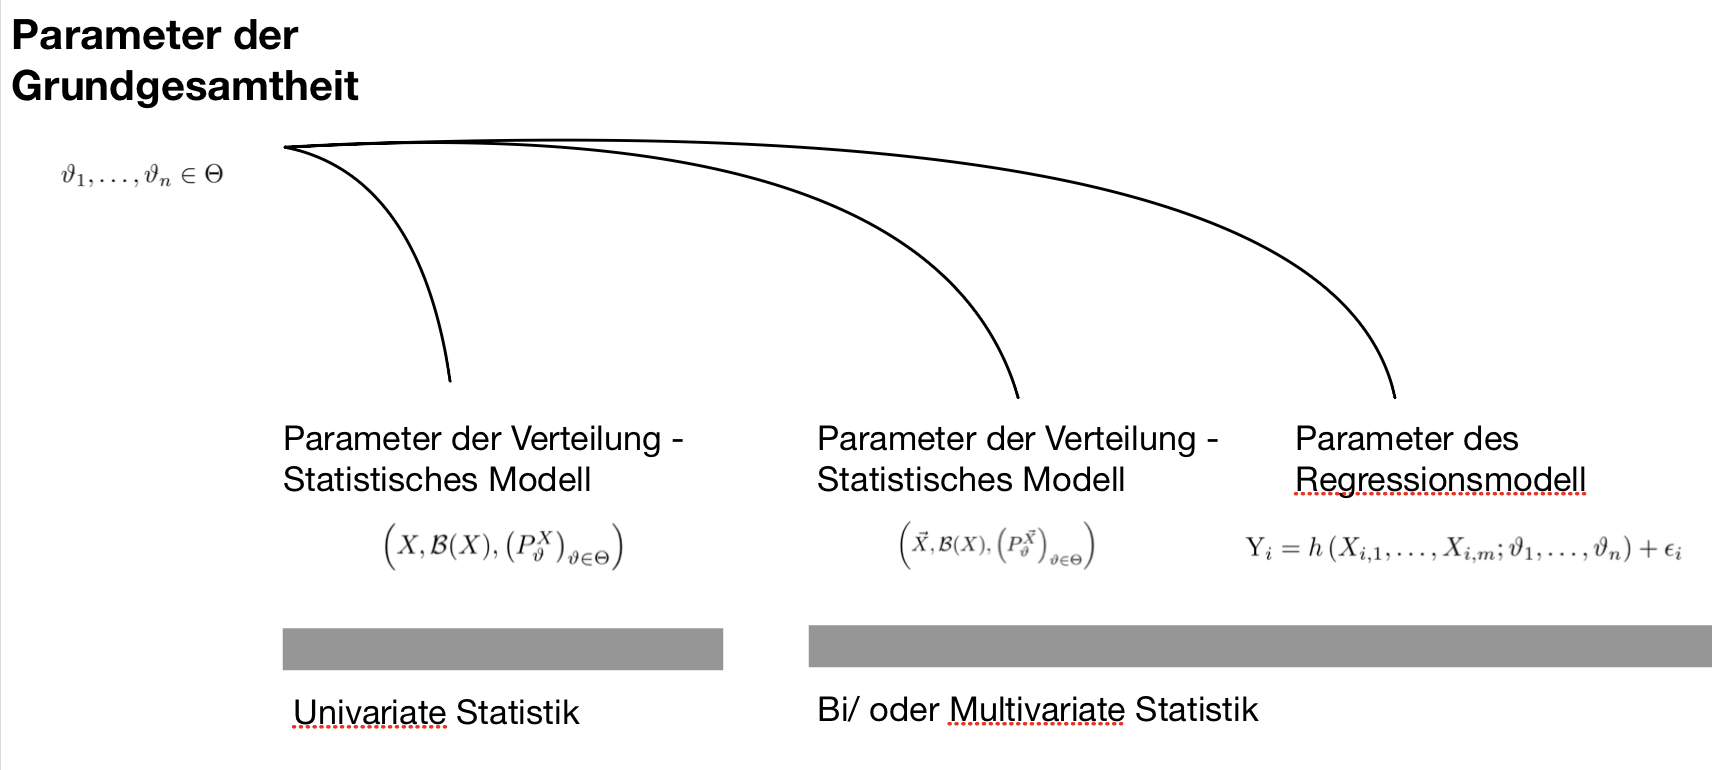
\includegraphics[width=0.7\linewidth]{attachment/chapter_13/Scc071}
	\caption{Parameter der Grundgesamtheit} 
\end{figure}

\subsection{Wahrscheinlichkeitsraum}
Zu beginn steht der \textit{Zufall}.\\

\begin{figure}[H]
	\centering
	
\includegraphics[width=0.7\linewidth]{attachment/chapter_13/Scc066}
	\caption{Gedanklicherprozess, um Zufall in geordnete Bahnen zu lenken.}
\end{figure}

Mit Hilfe des Konstrukt eines \gls{W.}Raums. Werden Ereignisse mit Wahrscheinlichkeiten versehen. Damit es mathematisch Kohärent ist, werden den einzelnen Elemente des Raums Eigenschaften abverlangt.

\begin{figure}[H]
	\centering
	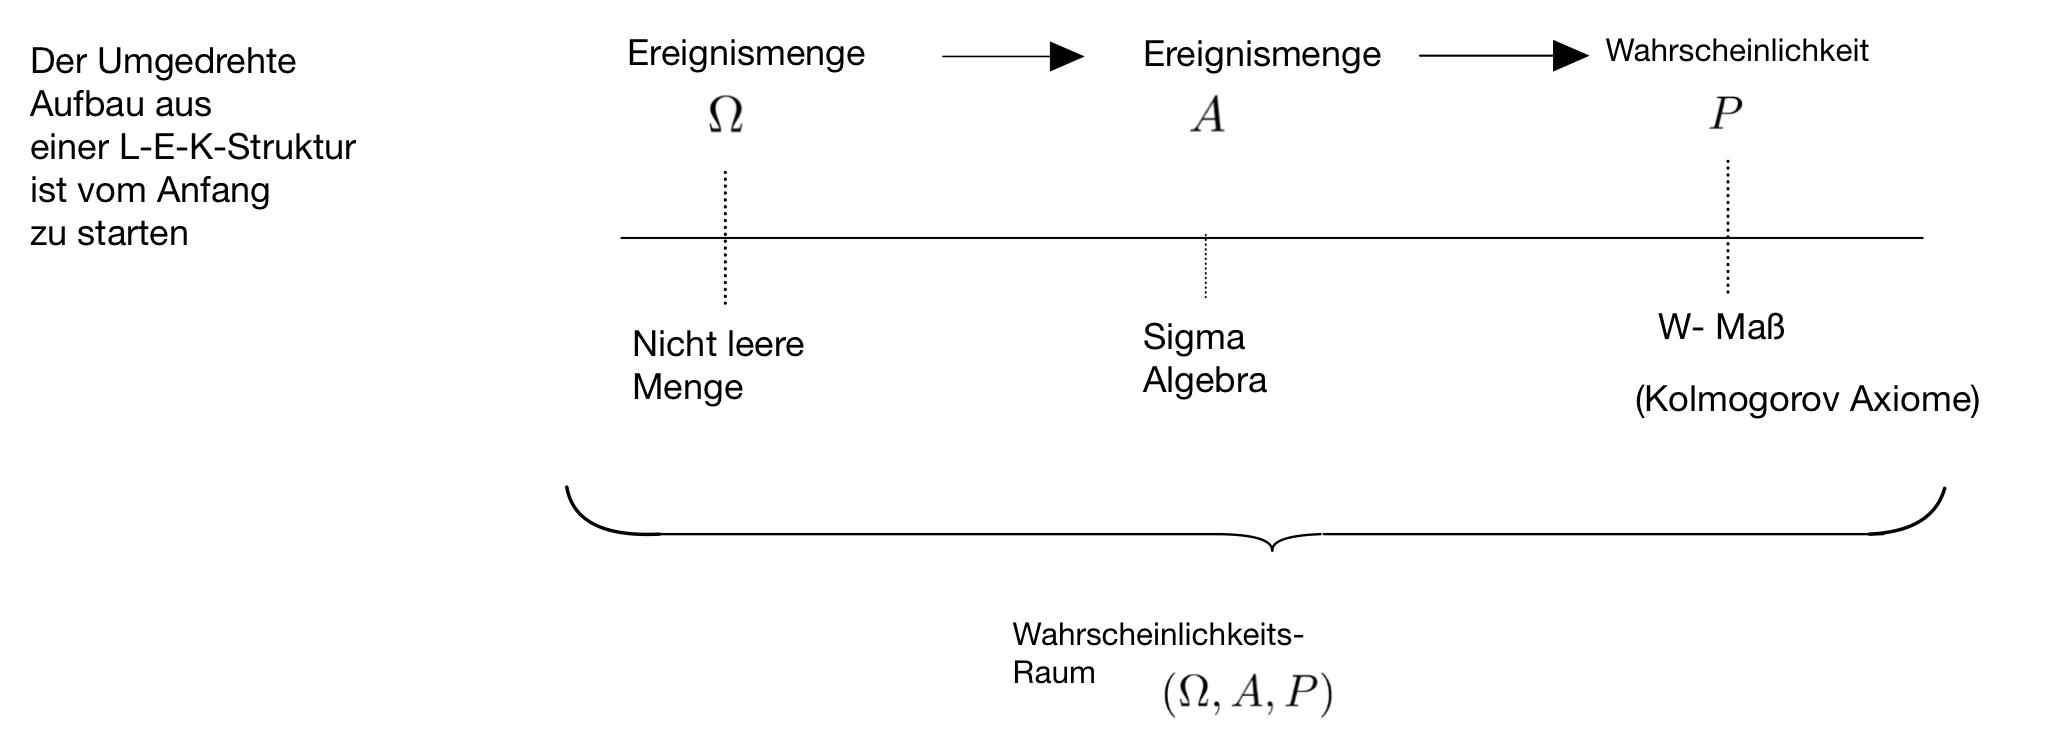
\includegraphics[width=0.7\linewidth]{attachment/chapter_13/Scc067}
	\caption{Der Wahrscheinlichkeitsraum}
\end{figure}

Auch hier gilt, das Problem mit dem gestartet wurde, wird ans Ende gestellt. Das L.E.K-Struktur lässt auch hier nicht direkt erkennen, was das Ziel von all dem Ausbau ist.

\subsection{Vererbung von Wahrscheinlichkeiten mit einer ZV}
\subsubsection{Mehrer Ausprägungen}
Angenommen es soll ein Würfelwurf modelliert werden. Dann wird benötigt
\begin{itemize}
	\item $\Omega = \Menge{1,2,3,4,5,6}$
	\item $\SigmaAlgebra = \Potenzmenge (\Omega) = \Menge{\emptyset,\Menge{1}, \Menge{1,2}, \dots}$
	\item $P(\Menge{\omega_i}) = \frac{1}{\#\Omega} = \frac{1}{6}$ \\
	Die anderen Elemente von $\SigmaAlgebra$ werden im Regelfall nicht aufgelistet, weil sie entweder implizit verstanden werden oder aus anderen Rechenregeln für Wahrscheinlichkeiten gelten. Als Beispiel für $P(\Menge{\emptyset})$ wird Null implizit verstanden. Für Ergebnisse, welche auch mehreren Ergebnissen $\omega$ bestehen, werden meist Rechenregeln angefügt oder implizit angenommen. Für diesen Fall wird jedem Element nichtleeren Element $\omega\in \Omega$ in $A\in \SigmaAlgebra$ die Wahrscheinlichkeit $\frac{1}{6}$ zugewiesen und diese addiert. Sodass gilt $P=\frac{3}{6}$, für $P(\Menge{1,2,3})$.
\end{itemize}

Die Zufallsvariable bildet die Ereignisse aus $\Omega$ auf $\R$ ab.

\begin{figure}[H]
	\centering
	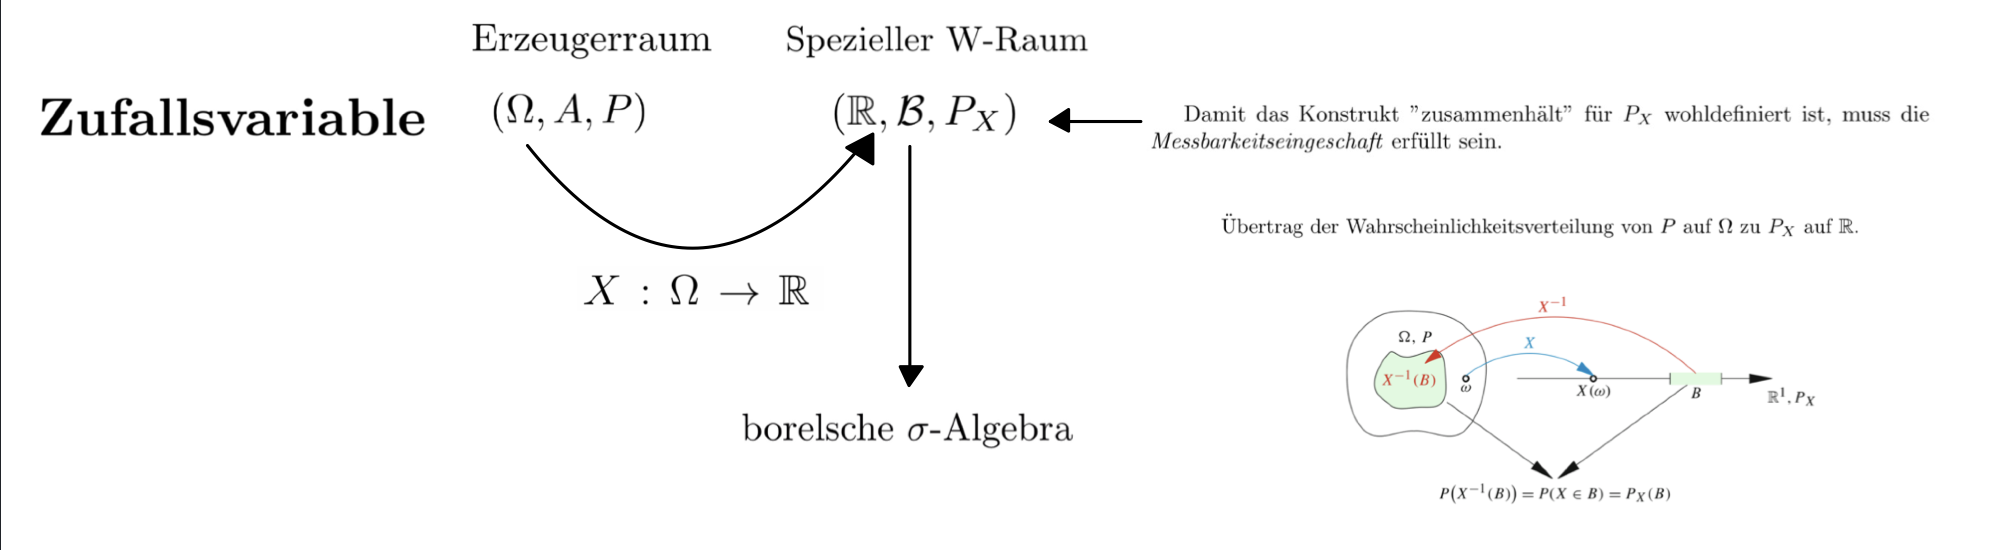
\includegraphics[width=0.7\linewidth]{attachment/chapter_13/Scc068}
	\caption{Neu Schaffung eines speziellen \WRaum}
\end{figure}

\paragraph{Einfacher Wurf eines Würfels}
Für diese Beispiel soll die Zufallsvariable eine obsolete Frage beantworten: 
\begin{align*}
	X:& \Omega \rightarrow \R, \omega \mapsto \omega \\
	& - \text{Augenzahl nach einem Wurf}
\end{align*}

Die Wahrscheinlichkeitfunktion $P_X$ definiert sich unter \refDefinition{Verteilung einer Zufallsvariable/ Wahrscheinlichkeitsfunktion}, und findet für $B= \Menge{1}\in \SigmaAlgebraIndividuel{B}$ 
\begin{align*}
	P_X(B) = P(X^{-1}(B))= P\left(\Menge{1}\right)=\frac{1}{6}
\end{align*}

\paragraph{Zweifacher Wurf eines Würfels}

Für zwei Würfel, welche geworfen werden gilt
\begin{itemize}
	\item $\Omega = \Menge{1,2,3,4,5,6}^2= \Menge{(1,1),(1,2), \dots}$
	\item $\SigmaAlgebra = \Potenzmenge (\Omega) = \Menge{\emptyset,\Menge{(1,1)}, \Menge{(1,1),(1,2)}, \dots}$
	\item $P(\Menge{\omega_i, \omega_j}) = \frac{1}{\#\Omega} = \frac{1}{36}$ für $\omega_i,\omega_j\in \Menge{1,2,3,4,5,6}$ Auch hier gilt, dass für die restlichen Elemente aus $\SigmaAlgebra$ Regeln oder Herleitungen impliziert angenommen oder durch die $\SigmaAlgebra$ definiert werden. Für das Beispiel $P(\Menge{(1,1),(2,1)})$ gilt $P(\Menge{(1,2)}) + P(\Menge{(2,1)}$. Dies leitet sich aus der $\SigmaAlgebra-\textit{additivit}$ her.
\end{itemize}

Auf diese $\Omega$ angewandt, werden hier drei verschiedenen Zufallsvariablen gebildet.
\begin{align*}
	X_1:& \Omega \rightarrow \R, (\omega_i,\omega_j) \mapsto min(\omega_i,\omega_j) \\
	& - \text{Geringste Augenzahl zwei Würfel}\\
	X_2:& \Omega \rightarrow \R, (\omega_i,\omega_j) \mapsto \omega_i+\omega_j \\
	& - \text{Summe der Augenzahl zweier Würfel}\\
	X_3:& \Omega \rightarrow \R, (\omega_i,\omega_j) \mapsto \omega_j\\
	& - \text{Zweite Augenzahl zweier Würfel}
\end{align*}
Durch die Messbarkeitseigenschaft \refDefinition{Verteilung einer Zufallsvariable/ Wahrscheinlichkeitsfunktion} wird auch hier die Wahrscheinlichkeit von $P$ übertragen. Für $X_2$ lässt sich $P_X$ grafisch aufzeigen.

\subsubsection{Einfache Ausprägung}

\paragraph{Münzwurf}
Für den \WRaum eines Münzwurfes, wird dieser wie folgt aufgespannt

\begin{itemize}
	\item $\Omega = \Menge{\textit{Kopf}, \textit{Zahl}}$
	\item $\SigmaAlgebra = \Potenzmenge (\Omega) = \Menge{\emptyset,\Menge{\textit{Kopf}}, \dots, \Menge{\textit{Kopf, Zahl}}}$
	\item $P(\Menge{\omega_i}) = \frac{1}{2}$
\end{itemize}

\paragraph{n-facher Münzwurf}
Für einen mehrfachen Münzwurf wird der \WRaum wie folgt aufgespannt

\begin{itemize}
	\item Für $i=1,2,\dots, n$ wird $\Omega_i = \Menge{1, 0}$ gesetzte.
	\item Für die $\SigmaAlgebra$  gilt $\SigmaAlgebra=\Potenzmenge(\Omega)$ mit $\Omega=\Omega_1\times \dots \times \Omega_n = \Menge{\omega = (\omega_1, \dots, \omega_n), \omega_i\in\Menge{0,1}}$
	\item $P(\Menge{\omega}) =  \prod P_i \left(\Menge{\omega_i}\right)$
\end{itemize}

Hierbei wird die Situation so abgebildet, das die Versucht

\paragraph{Binomial Verteilung aus Wahrscheinlichkeitsmaß}
Die gängigen Wahrscheinlichkeitsfunktionen für Zufallsvariablen wie Bernoulli, Poison oder ähnliche sind Funktionen, leitet sich aus dem Grundraum $(\Omega, \SigmaAlgebra, P)$ und der zu modellierenden Situation her. Die Wahrscheinlichkeitfunktion muss dabei ebenfalls die Messbarkeitseigenschaft einhalten.

Am Beispiel eines $n-$fachen Münzwurfs folgt. Sei $\omega = (\omega_1, \dots, \omega_n)\in \Omega$ ein beliebiges Elementarereignis gilt
\begin{align*}
	P\left(\Menge{\omega}\right) = \prod_{i:w_i=1} a_i \prod_{j:w_j=0}(1-a_j)
\end{align*}
mit $P_i(\Menge{1})=a$ und $P_i(\Menge{0})=1-a$, wobei mit einem \textit{identischen Versuchsaufbau} gilt $p_1=\dots p_n=p\in[0,1]$. Für eine bestimmte Anzahl $k=\left|\Menge{i:w_i=1}\right|$ von Ausprägungen von mit $1$ eines Elements, gilt für das Element $\omega\in \Omega$:
\begin{align*}
	P(\Menge{\omega}) = p^k(1-p)^{n-k}, \quad \forall k=0,1,\dots, n
\end{align*}

Um zu überprüfen, ob die Annahmen über die zu modellierenden Situation akkurat und zutreffen sind, kommt das Feld der Inferenzstatistik zum tragen.


	
\subsection{Dualität (Drei Faltigkeit) Input Zufallsvariable/Stichprobenwerte}
\label{subsec_Dualitaet_DreiFaltigkeit}
Im Umgang mit Schätzern, Statistiken und der Konstruktion von Zufallsvariablen ist die Dualität zwischen der theoretischen und realen Konstruktion dieser Abbildungen meist implizit angenommen. 

Als Beispiel, es werden selten beide Varianten einer Abbildung für eine Schätzfunktion notiert. Zum einen werden als Inputvariablen $X_1,\dots,X_n$ verwendet, zum anderen $x_1,\dots,x_n$ als Realisation der Stichprobe.

\begin{figure}[H]
	\centering
	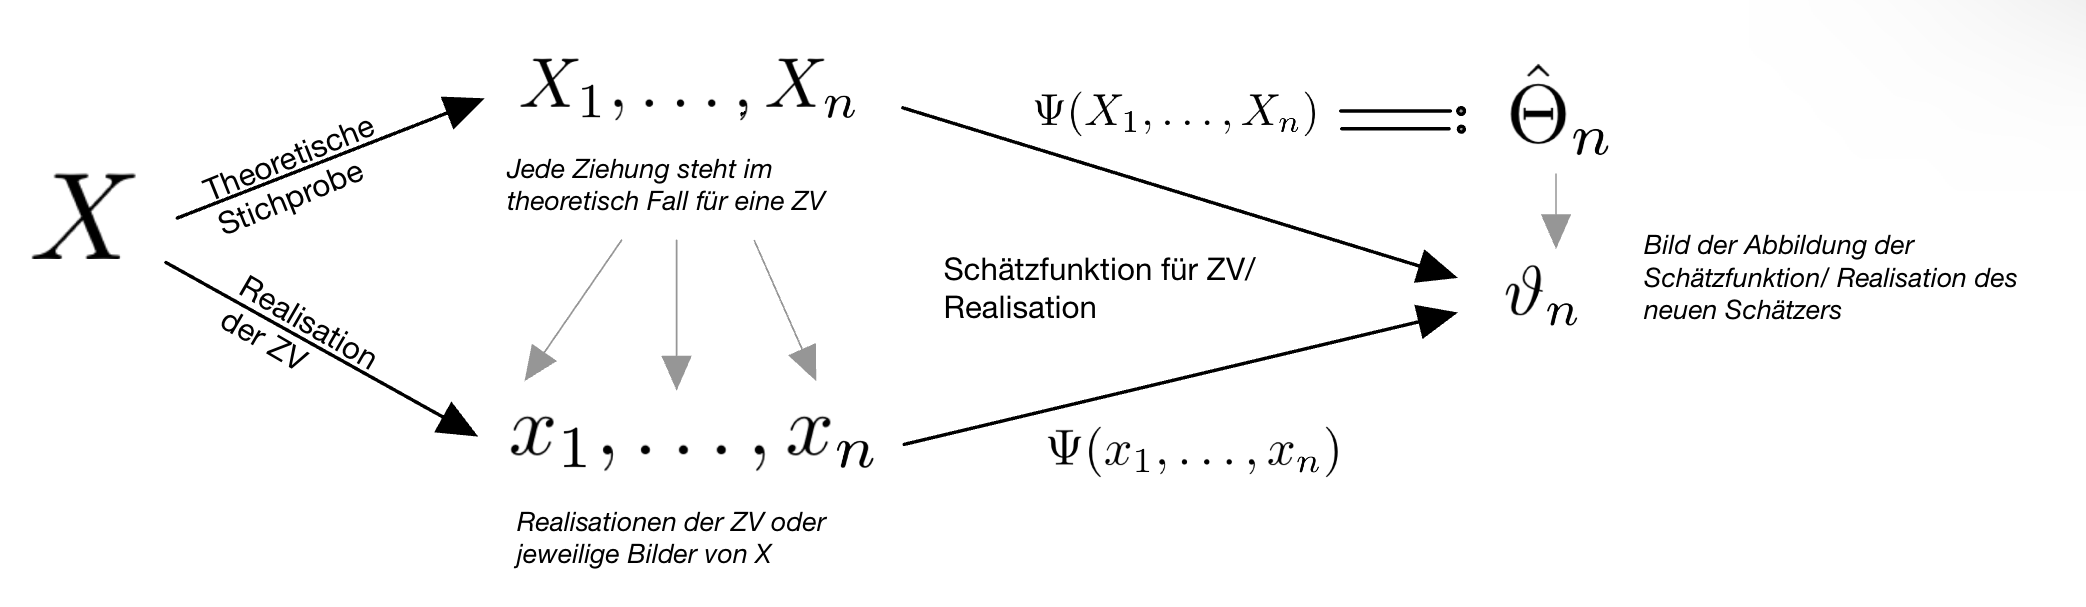
\includegraphics[width=0.7\linewidth]{attachment/chapter_13/Scc072}
	\caption{Dualität - Theoretischer und Realisationsverlauf}
\end{figure}

Es besteht ein weiter Zusammenhang zwischen der 
\begin{itemize}
	\item tatsächlichen Abbildung, der Schätzfunktion,
	\item der neuen Konstruktion einer \gls{ZV} und
	\item der tatsächlichen Realisation, als Schätzwert für den Parameter oder die Parameterfunktion
\end{itemize}

\begin{figure}[H]
	\centering
	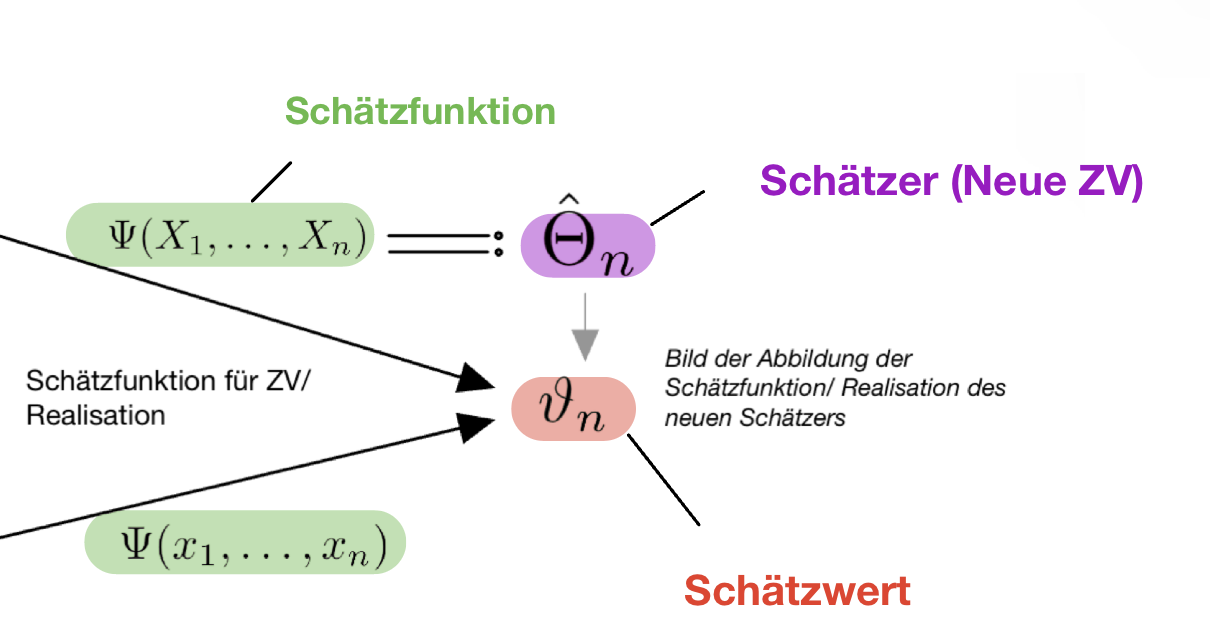
\includegraphics[width=0.7\linewidth]{attachment/chapter_13/Scc073}
	\caption{Drei Faltigkeit - Schätzer, Schätzfunktion und Schätzwert}
\end{figure}

\subsection{Abriss Deskriptive Statistik}

In der Deskriptiven Statistik wird der Gesichtpunkt geändert. Die Realisationen der Zufallsvariablen liegen vor. Es wird jetzt kein Rückschluss auf die wahren \gls{W.}Raum gezogen, sondern eher eine Bewertung und Darstellung der Daten vollzogen. 
\begin{center}
	Achtung: Die Begrifflichkeiten spiegeln sich und es gibt viele Gleichheiten. Es handelt sich aber hier nicht um das Feld der Induktiven Statistik.
\end{center}

Wie schon erwähnt, gibt es ähnliche Konzept, welche sich \underline{schwach} zuordnen.
\begin{table}
	\begin{tabular}{ll}
		Merkmal $X$ & Zufallsvariable $X$ \\ \hline
		$\Omega$ ist die Grundgesamtheit & $\Omega$ ist die Ergebnismenge und gehört zu einem \gls{W.}Raum \\
		$M$ ist der Merkmalsraum & $\R$ ist Bildraum \\
		$X(\omega)$ ist die Ausprägung & $X(\omega)$ ist die Realisation \\
		$X$ besitzt eine Häufigkeitsverteilung & $X$ besitzt eine \gls{W.} Maß (\gls{W.}verteilung) \\
		$X$ besitzt eine empirische Verteilungsfunktion & $X$ besitzt eine theoretische Verteilungsfunktion
	\end{tabular}
\end{table}

\paragraph{Merkmal vs Zufallsvariable}
Anders als im vorherigen Kapitel ist ein Merkmal zwar das Kernelement der Despriptiven Statistik, jedoch nicht so strikt definiert wie die Zufallsvariable. Der Begriff der \gls{ZV} wird jedoch oft als Synonym verwandt.
\begin{Definition}{Merkmal}
	Ein \textit{Merkmal} ist eine Abbildung von $\Omega$ in eine Menge $M$:
	\begin{align*}
		X : \Omega \rightarrow M
	\end{align*}
	Wenn die Menge $M$ ohne weitere Struktur ist, so ist $X$ ein \textbf{nominales Merkmal}. Ist $X(\Omega)$ eine geordnete Menge, so ist $X$ ein \textbf{ordinales Merkmal}. Ist $X(\Omega)\subset \R$ und übernimmt die $X(\Omega)$ die euklidische Metrik, so ist $X$ ein \textbf{quantitatives} oder \textbf{kardinales} Merkmal.
\end{Definition}
Die Skalierung von Merkmalen erlaubt Vergleichsmöglichkeiten:
\begin{description}
	\item[Nominal] $X(\omega_1) = X(\omega_2)$ oder $X(\omega_1) \neq X(\omega_2)$
	\item[Ordinal] $X(\omega_1) \preceq X(\omega_2)$ oder $X(\omega_1) \simeq X(\omega_2)$
	\item[Kardinal] $X(\omega_1) - X(\omega_2)$
\end{description}